\documentclass[]{article}
\usepackage{graphicx}
\usepackage{xcolor}
\usepackage{float}
\usepackage{amsmath, commath}
\usepackage{hyperref}
\hypersetup{
	colorlinks=true,
	linkcolor=cyan,
	filecolor=magenta,      
	urlcolor=blue,
}
\usepackage{color}
\usepackage{listings}
\lstdefinestyle{mystyle}{
	% backgroundcolor=\color{backcolour},   
	commentstyle=\color{orange},
	keywordstyle=\color{blue},
	numberstyle=\tiny\color{gray},
	stringstyle=\color{purple},
	basicstyle=\footnotesize,
	breakatwhitespace=false,         
	breaklines=true,                 
	captionpos=b,                    
	keepspaces=true,                 
	% numbers=false,                    
	numbersep=5pt,                  
	showspaces=false,                
	showstringspaces=false,
	showtabs=false,                  
	tabsize=2
}
\lstset{style=mystyle}
\usepackage{indentfirst}

%opening
\title{A Critique of \textit{Testing Theories of American Politics: Elites, Interest Groups, and Average Citizens} \cite{gilens}}
\author{Michael T Da Silva\footnote{\href{mailto:mdasilva@callutheran.edu}{mdasilva@callutheran.edu}}, Peter Cramer}

\begin{document}
\maketitle

\begin{abstract}
	The conclusion drawn in \textit{Testing Theories of American Politics: Elites, Interest Groups, and Average Citizens} -- the legislation passed in the U.S. is uninfluenced by the opinion of those not in the economic elite or business-oriented special interest groups -- is supported by figures and tables which misrepresent the data. Upon reevaluation, it appears that there are insufficient data for the multivariate model used to differentiate between the three groups examined.
	
	Additionally, there are critical defects with figures and statistics which, taken together with the failure to replicate the multivariate model, lead us to the conclusion that the original paper should be retracted.

\end{abstract}

\section{Motivation and Outline of Critique}
Rhetoric surrounding voting is becoming increasingly heated in the U.S. \cite{voting_rights}. 
As such, an influential paper which has a figure which can be interpreted to mean that voting has no impact on policy adoption if one is not in the top 90th percentile of income or aligned with powerful interest groups is a potential political flash-point.

This analysis will begin with a close inspection of the model used by examining the tables given in the original paper.
Then, we will attempt to regenerate the model in question to elucidate what methods were used to create it and what assumptions were baked in.
Finally, the narrative and conclusions will be examined in light of the model and tables.\\

The Python and data used in this analysis can be found on Github at \href{https://github.com/ChemistryMickey/testing-theories-of-american-politics-data-analysis}{testing-theories-of-american-politics-data-analysis}. Additionally found there is an R script provided by the authors (though used in a separate paper for a similar analysis but given as an example of their process). The software used for the authors' analysis was IBM's Amos package such that more tailored statistical analysis may have been performed but if so, we will here show that it was not properly communicated.

\section{Acknowledgments}
Thank you to Dr. Martin Gilens for providing additional analysis scripts and data clarification as well as Drs. Martin Gilens and Benjamin Page for collecting these data. 
It clearly took a massive amount of work to gather and process.
Thank you also for making them available at \cite{gilens}.

Thank you also to Drs. Dhindsa and Patel for the additional sanity check.

\newpage
\section{Tables 3 \& 4 - p-scores and $R^2$}
To begin, we will explore tables 3 and 4 which relate to both theoretical economic models outlined in the paper and the data.
For more information on the economic models themselves, refer to the paper but the criticism contained herein is comprehensible without an understanding of them.
For a brief refresher on p-scores and $R^2$ values, please refer to sections \ref{section_p-score} and \ref{section_R-sq} respectively.

\begin{figure}[H]
	\begin{center}
		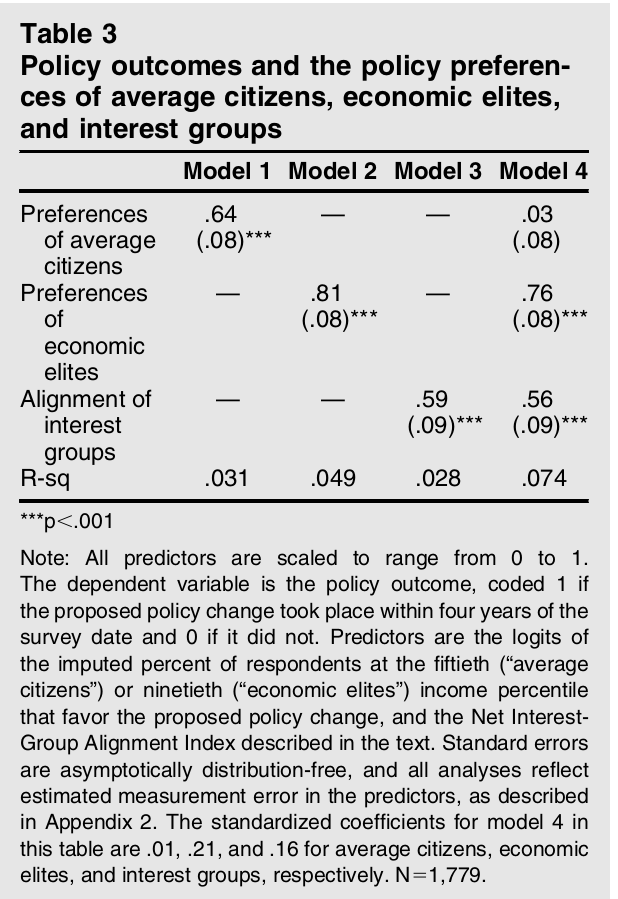
\includegraphics[height=300px]{./figures/paper/economic-table3.png}
	\end{center}	
	\caption{Table 3 from \textit{Testing Theories of American Politics: Elites, Interest Groups, and Average Citizens} is here shown. The same criticism will be levied against both tables 3 and 4 such that repeating it twice is counterproductive. Please refer to table 4 (figure \ref{paper_table4}) for the full critique but it applies equally here.}
	\label{paper_table3}
\end{figure}

\begin{figure}[H]
	\begin{center}
		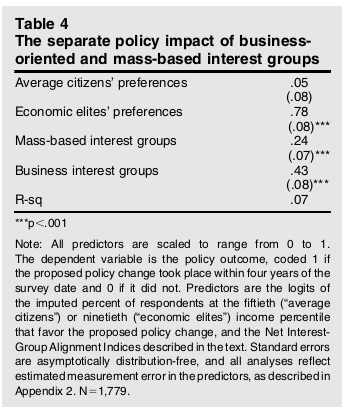
\includegraphics[height=300px]{./figures/paper/economic-table4.png}
	\end{center}	
	\caption{Table 4 from \textit{Testing Theories of American Politics: Elites, Interest Groups, and Average Citizens} is here shown. In particular we should focus on two numbers on this table: $p < .001$ and R-sq ($R^2$) $= 0.07$. Briefly, p-score is a measure of how confident one can be that their measurement is within a distribution (the lower, the more likely it is from a \textit{different} distribution; this is the desired condition to prove significance), and $R^2$ is a measure of how well a model fits data (the closer to 1 the better the fit). As such, having a p-score so low (which indicates high confidence) and an $R^2$ of nearly zero (which indicates no correlation), we can be confident that the model used to generate this table fails to capture trends in the data. \\With that, we cannot draw any further conclusions from tables 3 or 4. Unfortunately, these tables are critical for the authors' arguments such that they cannot be used as proof and may even contradict the authors' conclusion.}
	\label{paper_table4}
\end{figure}

To further emphasize this point, figure \ref{generated_low_r2} demonstrates data that has an $R^2$ of a similar value as these tables but is obviously a poor fit.
\begin{figure}[H]
	\begin{center}
		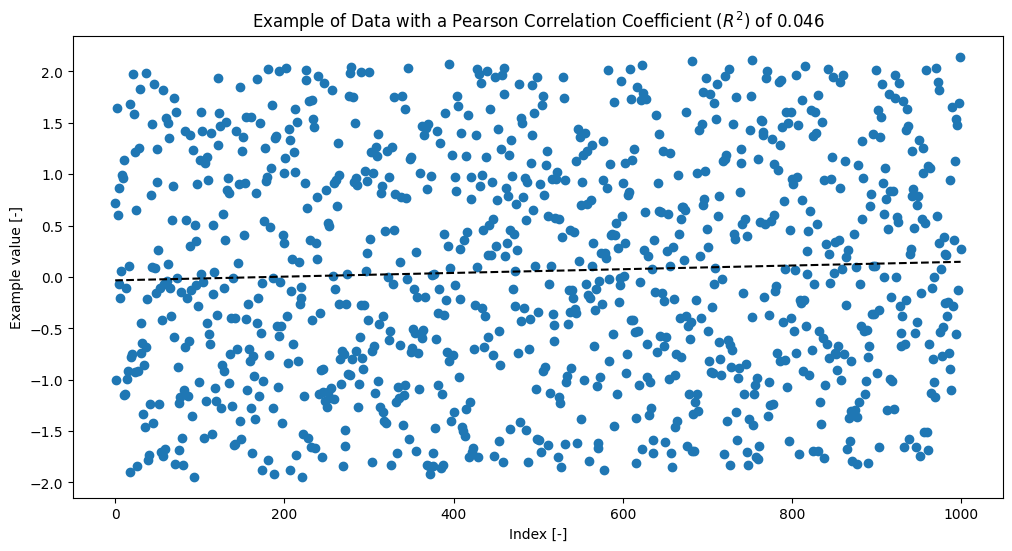
\includegraphics[width=300px]{./figures/generated/example-low-r2-plot.png}
	\end{center}	
	\caption{Example randomly generated data with an $R^2$ on par with those found in tables 3 and 4 are here shown. Hopefully it is plain to see that concluding the fitted line (black dotted) is a good representation of the data is false. For further info on $R^2$ values, their meaning, and calculation, please refer to section \ref{section_R-sq}.}
	\label{generated_low_r2}
\end{figure}

\section{Attempted Model Regeneration}
\label{section:model-regen}
\subsection{Regenerating Exactly as Defined in Author-Provided R Script}
In communicating with Dr. Martin Gilens, an R script was provided which includes a Structural Equation Model (SEM) which ostensibly reproduces the results obtained in the original paper.
This model was run in both R (using Lavaan \cite{lavaan}) and Python (using semopy \cite{semopy}) and the result obtained was nothing close to that expressed in tables 3 and 4 of the original paper.

The model used in both cases is the following (here in python):
\begin{lstlisting}[language=python,label=strict-model-definition,caption={SEM model with assumed, manual covariance between rangepred50 and rangepred90}]
from semopy import Model
model = Model(
	description="""
		# measurement
		L5 =~ 1 * rangepred50
		L9 =~ 1 * rangepred90
		IG_bal =~ 1 * rangeinterest
		
		# regressions
		policy_change ~ L5 + L9 + IG_bal
		
		# cov and var
		rangepred50 ~~ 0.0026380 * rangepred90
		L5 ~~ IG_bal
		L9 ~~ IG_bal
		L5 ~~ L9
	""",
	mimic_lavaan=True,
)	
\end{lstlisting}
where
\begin{enumerate}
	\item L5 is a name substitution for rangepred50 which is the normalized and logistical quartile probability of policy adoption for the 50th percentile given by the following transformations: 
	\begin{lstlisting}[language=python]
		rangepred50 = normalize(qlogis(raw_data["pred50_sw"]))
	\end{lstlisting}
	where "normalize" is given by the simple equation $\tilde{x} = \frac{x - \min(x)}{\max(x) - \min(x)}$, "qlogis" \cite{R-logistic} is the slightly more complex $$\text{qlogis}(x) = \frac{1}{1 + e^{-\frac{x - \mu}{\sigma}}}$$ and "pred50\_sw" is the proportion of the 50th economic percentile in favor of the piece of legislation passing -- calculated per-piece of legislation. In this case, $\mu$ and $\sigma$ are assumed to be 0 and 1 respectively\footnote{This may be a bad decision because it means all data vectors to which this is applied will be mapped to something gaussian-like and then normalized which sounds like it introduces artificial similarity. Normalization is necessary for the multivariate analysis but the additional use of "qlogis" with $[\mu, \sigma] = [0, 1]$ may be erroneous.}.
	\item L9 is a name substitution for rangepred90 which is transformed identically to L5.
	\item IG\_bal is a name substitution for rangeinterest which is calculated using the following equation\footnote{This equation visually differs from that defined in the original paper, but using the log rule $\ln(a/b) = \ln(a) - \ln(b)$, we can obtain this slightly shorter equation.}:
	\[\text{net interest group alignment} = \ln\Big(\frac{\text{\# Strongly favor} + \frac{1}{2} \text{\# Weakly favor} + 1}{\text{\# Strongly oppose} + \frac{1}{2} \text{\# Weakly oppose} + 1}\Big)\]
	This "net interest group alignment" is then normalized between 0 and 1 to yield IG\_bal:
	\[ \text{IG\_bal} = \text{normalize}(\text{net interest group alignment}) \]
	\item policy\_change is declared to be a function of L5, L9, and IG\_bal
	\item rangepred50 is declared to have an artificially small dependence on rangepred90 (e.g. if rangepred90 changes by 1, this line asserts that rangepred50 should change 0.0026380)\footnote{At least the optimizer should start with this assumption; it is allowed to optimize away from this relationship).}. This is asserting the conclusion that rangepred90 is the more significant factor. Despite that artificial assumption, we will see in figure \ref{strict-regen-multivariate-correlation} that it still does not regenerate the result obtained in the original paper's tables 3 and 4 and the optimizer finds the contradictory conclusion.
	\item L5 is defined to be correlated with IG\_bal
	\item L9 is defined to be correlated with IG\_bal
	\item L5 is defined to be correlated with L9
\end{enumerate}
When this is run, the following relationships between the three variables (L5, L9, IG\_bal) are obtained:
\begin{figure}[H]
	\begin{center}
		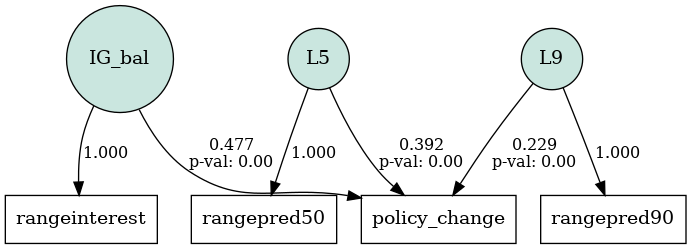
\includegraphics[width=\linewidth]{./figures/generated/multivariate-analysis/strict-regen-multivariate-correlation.png}
	\end{center}
	\caption{An attempt at regenerating the multivariate model used in \textit{Testing Theories of American Politics: Elites, Interest Groups, and Average Citizens} is here shown. Please see listing \ref{strict-model-definition} for a definition of the model and the corresponding explanation for variable name descriptions. The arrows, however, signify the following:\\ - IG\_bal (i.e. interest groups) has the largest influence on the probability of policy change adoption (0.477)\\- L5 (i.e. the 50th income percentile) has middling influence on the probability of policy adoption (0.392)\\- L9 (i.e. the economic elite) has the smallest influence on the probability of policy adoption (0.229)\\This contradicts the conclusion of the original paper.\\It should be noted, however, that wherever an optimizer is involved, many results may follow. It is unclear how IBM's AMOS package may have optimized this. It does, however, show that the result is likely an artifact of how few data are present.}
	\label{strict-regen-multivariate-correlation}
\end{figure}

A more complete look at the relationships between these three variables also shows the most critical feature:
\begin{figure}[H]
	\begin{center}
		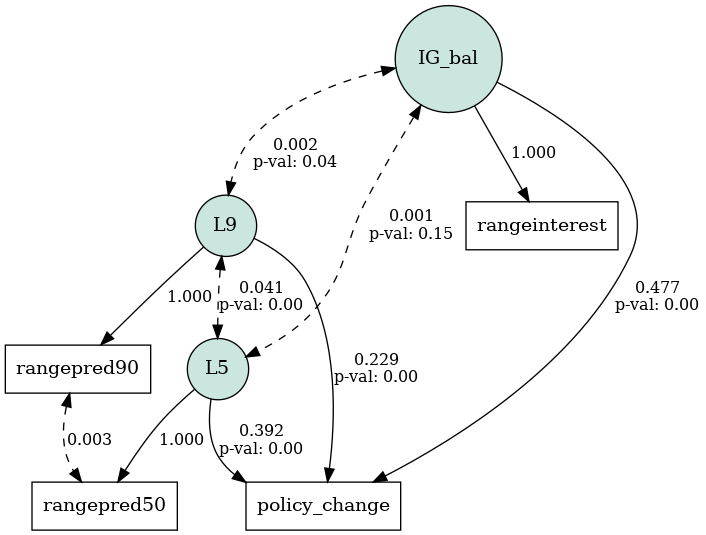
\includegraphics[width=\linewidth]{./figures/generated/multivariate-analysis/strict-regen-multivariate-correlation-full.png}
	\end{center}
	\caption{An more complex relationship plot for the model generated in figure \ref{strict-regen-multivariate-correlation} is here shown. Please see listing \ref{strict-model-definition} for a definition of the model and the corresponding explanation for variable name descriptions. \textbf{The critical observation to make here is that the p-val for the relationship between L5 and IG\_bal is quite large (0.15) such that we cannot conclude that they are separate distributions.} As such, this model fails to differentiate between the policy preferences of the 50th percentile and interest groups (at least in the way the data have been preprocessed).}
	\label{strict-regen-multivariate-correlation-full}
\end{figure}

In conclusion, the model as defined in the R script provided by Dr. Martin Giles fails to reproduce the model used in the generation of figure 1 and tables 3 and 4 of the original paper. Additionally, the model here developed has insufficient data to differentiate between the groups under examination such that it is unlikely that, even with RNG cherry-picking, it is possible to draw a substantial conclusion

Without that model, the result of the paper is unsubstantiated.

\subsection{Regenerating without Assumed Covariance}
Removing the manually assumed covariance from listing \ref{strict-model-definition}, we obtain the following model:
\begin{lstlisting}[language=python,label=no-covariance-model-definition,caption={SEM model without assumed covariance between rangepred50 and rangepred90}]
from semopy import Model
model = Model(
	description="""
		# measurement
		L5 =~ 1 * rangepred50
		L9 =~ 1 * rangepred90
		IG_bal =~ 1 * rangeinterest
		
		# regressions
		policy_change ~ L5 + L9 + IG_bal
		
		# cov and var
		L5 ~~ IG_bal
		L9 ~~ IG_bal
		L5 ~~ L9
	""",
	mimic_lavaan=True,
)	
\end{lstlisting}
Using this model, a similar result to figure \ref{strict-regen-multivariate-correlation-full} is obtained:
\begin{figure}[H]
	\begin{center}
		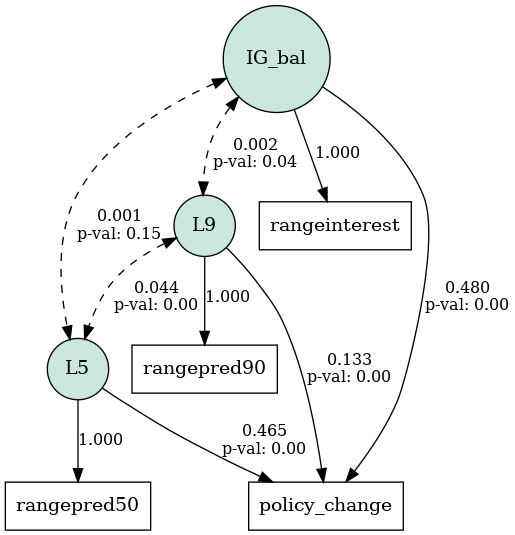
\includegraphics[width=200px]{./figures/generated/multivariate-analysis/no-assumed-covariance-multivariate-correlation-full.png}
	\end{center}
	\caption{The model result from listing \ref{no-covariance-model-definition} is here shown. Please see listing \ref{no-covariance-model-definition} for a definition of the model and the corresponding explanation for variable name descriptions from listing \ref{strict-model-definition}. \textbf{Here we can see again (w.r.t. figure \ref{strict-regen-multivariate-correlation-full}), that L5 and IG\_bal cannot be differentiated and they both have a much more significant impact on the probability of policy adoption than L9.}}
	\label{no-covariance-regen-multivariate-correlation-full}
\end{figure}

In conclusion, even the assumed covariance between rangepred50 and rangepred90 cannot explain the model obtained by the authors in the original paper; it is possible that manipulating the RNG seed could lead to the authors' original conclusion but even if such RNG-hacking were used, because L5 and L9 are so strongly correlated in the original dataset, it is likely that the p-value which currently marks IG\_bal and L5 as undifferentiable would instead show IG\_bal and L9 to be undifferentiable.

\section{Inspection of Figure 1}

\begin{figure}[H]
	\begin{center}
		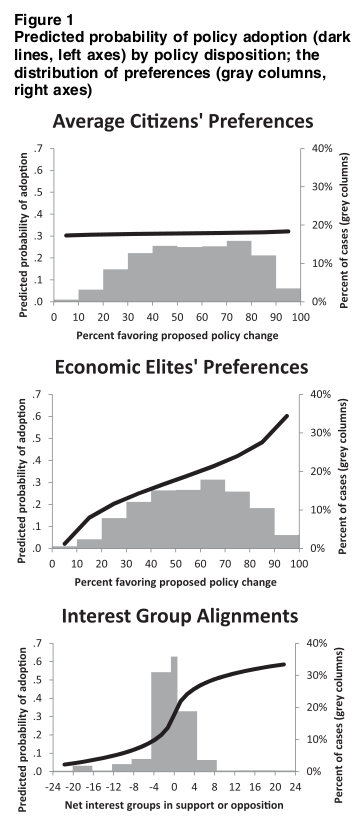
\includegraphics[height=400px]{./figures/figure1.png}
	\end{center}	
	\caption{Figure 1 from \textit{Testing Theories of American Politics: Elites, Interest Groups, and Average Citizens} is here shown. From a clarity standpoint, figures should, ideally, be able to stand by themselves because they are most likely to be taken out of context. As such, a more comprehensive figure caption would be appreciated such that the narrative is clearly explained along with the analysis method performed to generate these plots.}
	\label{paper_figure1}
\end{figure}

To begin, we must understand how this figure was generated.
Based on page 572R, these figures were created using the multivariate model.
In the previous sections, however, we have shown that the multivariate model is either deeply flawed or misleading.
As such, we should be able to discount figure 1 immediately but upon closer inspection, additional concerns are raised.

\subsection{Figure 1a - Average Citizens' Preferences}
\begin{figure}[H]
	\begin{center}
		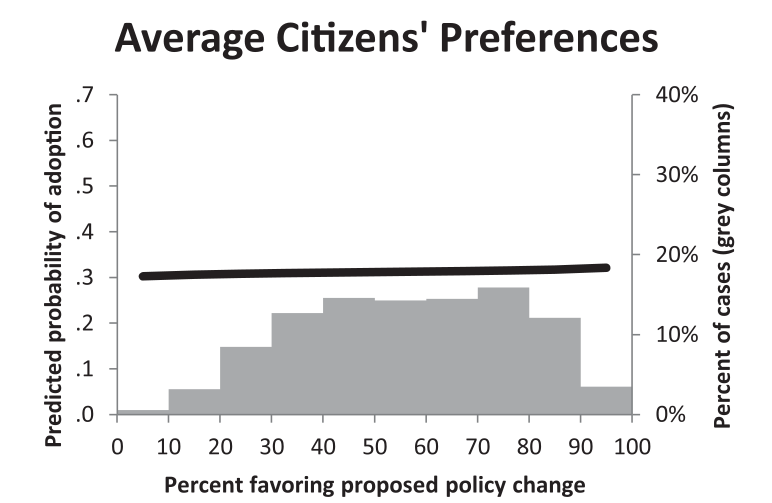
\includegraphics[width=300px]{./figures/paper/average-citizens-preferences.png}
	\end{center}	
	\caption{Figure 1a from \textit{Testing Theories of American Politics: Elites, Interest Groups, and Average Citizens} is here shown. An explanation of the axes follows: \\The x-axis is the proportion of people in this income percentile (here the 50th percentile) who want the legislation to pass; the 90-100 bracket therefore indicates that 90-100\% of survey respondents in the 50th income percentile want the legislation to pass. \\The left axis indicates the probability that the legislation will pass for that preference bracket; if 90-100\% of 50th income percentile want legislation to pass, this plot indicates there is a slightly greater than 30\% chance of it passing. \\The right axis indicates the number of cases examined in this dataset which have that proportion of 50th income percentile respondents favoring the policy being adopted; out of these $\approx$1800 cases examined, about 4\% of them had 90-100\% of the 50th income percentile favoring their adoption.}
	\label{paper_figure1a}
\end{figure}

Nothing about this figure immediately stands out as problematic beyond the model that is used to generate it. There is a reasonable distribution of cases (see figure \ref{paper_figure1a} for an explanation of axes) across percent favoring brackets and it is approximately normal.


\subsection{Figure 1b - Economic Elites' Preferences}
\label{section_figure1b}
\begin{figure}[H]
	\begin{center}
		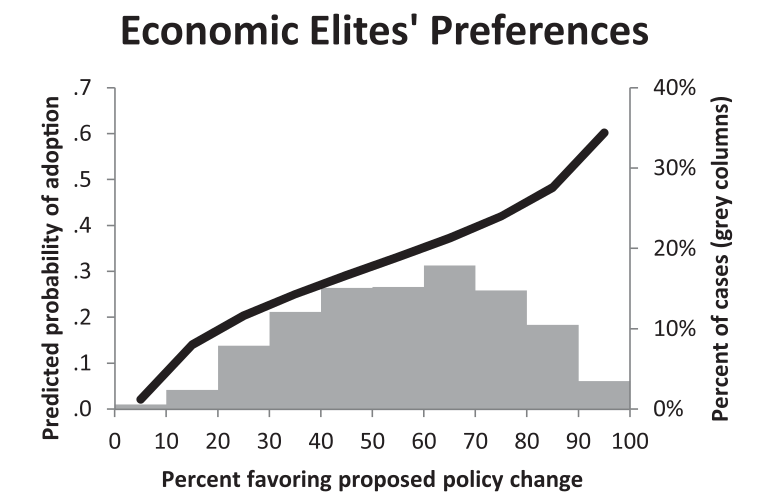
\includegraphics[width=300px]{./figures/paper/economic-elites-preferences.png}
	\end{center}	
	\caption{Figure 1b from \textit{Testing Theories of American Politics: Elites, Interest Groups, and Average Citizens} is here shown. Here we can plainly see (in contrast to figure \ref{paper_figure1a}) that as more economic elites prefer adopting a policy, the greater the chance that policy is adopted.}
	\label{paper_figure1b}
\end{figure}

Nothing about this figure immediately stands out as problematic beyond the model that is used to generate it.


\subsection{Figure 1c - Interest Group Alignments}
\begin{figure}[H]
	\begin{center}
		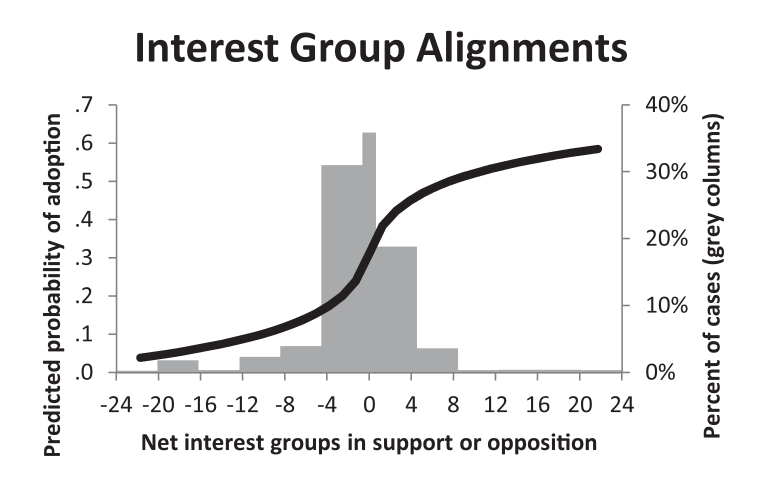
\includegraphics[width=300px]{./figures/paper/interest-group-preferences.png}
	\end{center}	
	\caption{Figure 1c from \textit{Testing Theories of American Politics: Elites, Interest Groups, and Average Citizens} is here shown. Without delving into the text, several issues stand out. \\The data are approximately normal about 0 but the plot extends beyond where there are data. A plot between [-6, 6] would have been sufficient to hypothesize that interest group alignment is correlated with legislative outcome without extrapolating into a sparse or absent data region. \\Given how few data are in some regions, even though this is the output of a multimodal model, this is clearly impossible. The choice of a logistic/sigmoid function for this interpolation/extrapolation additionally encodes an assumption which may not be valid. \\Additionally, the equation for net interest groups as given on page 569R of the original paper (shown in section \ref{section:model-regen} and included again below this caption), cannot have been here used. That equation simplifies to $\text{Net Interest Group Alignment} = \ln(a/b)$ where $a$ and $b$ are functions of how many interest groups support, $a$, or oppose, $b$, a policy. If we examine the extrema of the axes, $[e^{-24}, e^{24}] \approx [0, 2.6E^{10}]$. There are not $2.6E^{10}$ humans on Earth, nevermind interest groups even if we double them for being strongly in favor or opposed. Even within the center of highest density, $e^{4} \approx 54$ is a greater additive favor score, $a$, than any policy received in the dataset.\\As a final sanity check for the data distribution, please find a histogram of the net interest group calculated as a simple sum in figure \ref{generated_figure1c_data_sparsity}.}
	\label{paper_figure1c}
\end{figure}

The equation ostensibly used in the generation of the x-axis for figure \ref{paper_figure1c} follows:
\begin{align*}
	\text{Net Interest Group Alignment} &= \ln(\text{\# Strongly Favor} + 0.5 * \text{\# Somewhat Favor} + 1) \\&- \ln(\text{\# Strongly Oppose} + 0.5 * \text{\# Somewhat Oppose} + 1) \\&= \ln\Big(\frac{\text{\# Strongly Favor} + 0.5 * \text{\# Somewhat Favor} + 1}{\text{\# Strongly Oppose} + 0.5 * \text{\# Somewhat Oppose} + 1}\Big) \\&= \ln(a/b)
\end{align*}
See figure \ref{paper_figure1c}'s caption for an explanation of why this cannot have been used in figure \ref{paper_figure1c}.

\begin{figure}[H]
	\begin{center}
		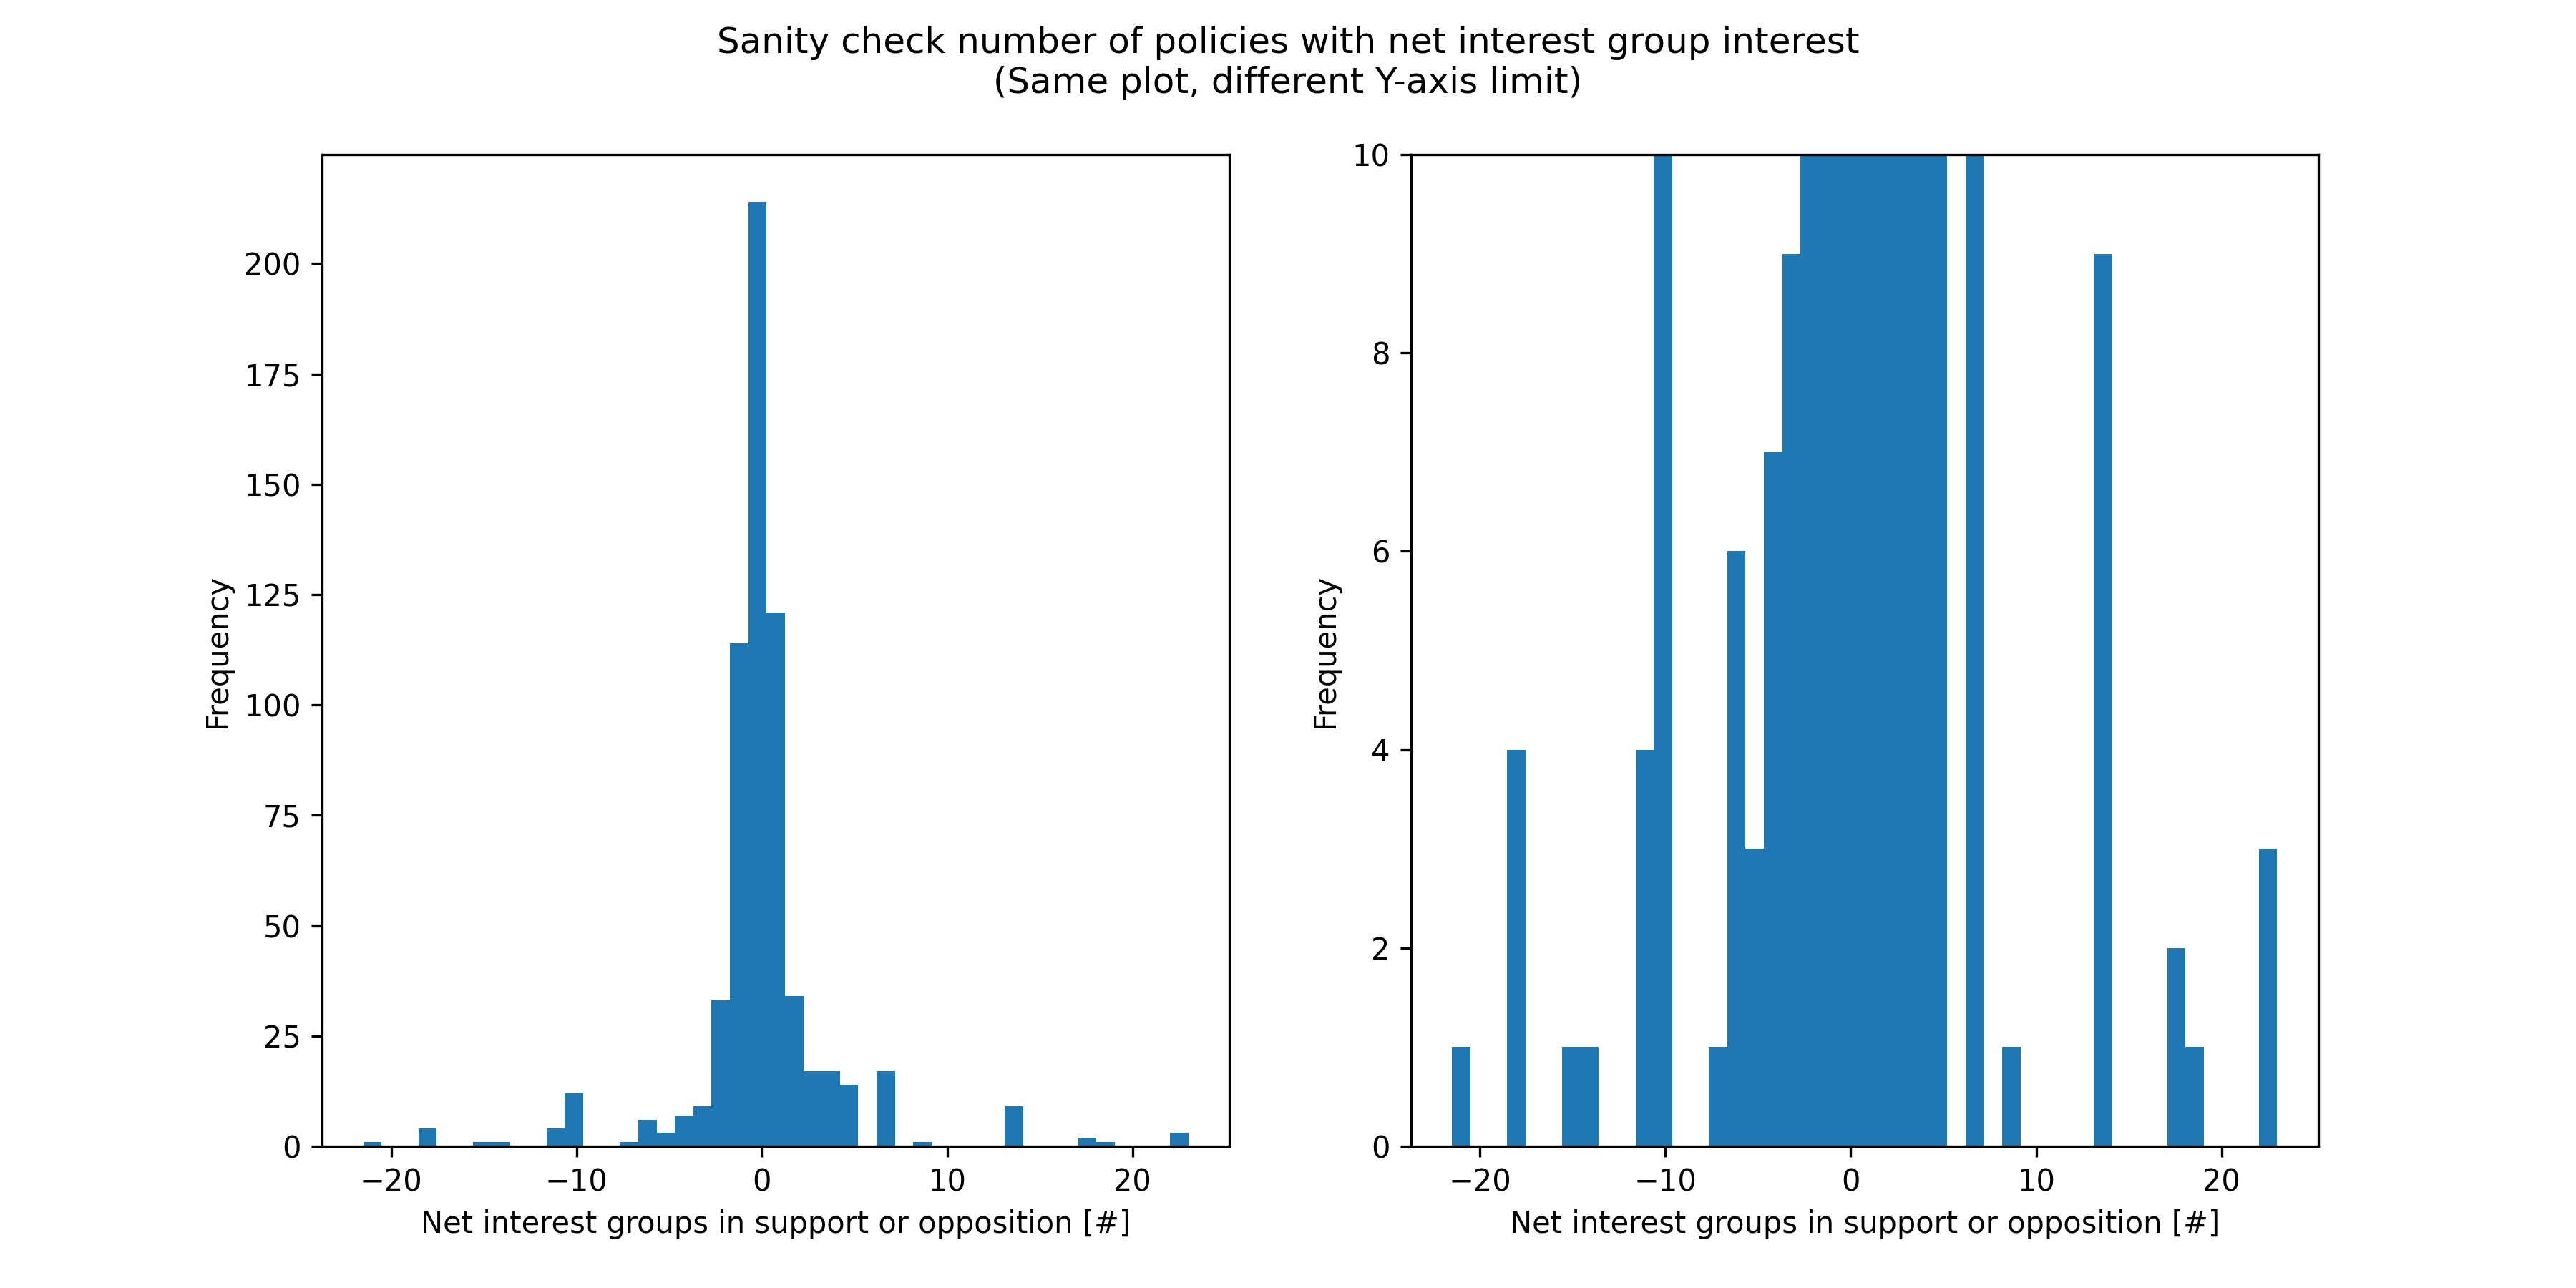
\includegraphics[width=300px]{./figures/generated/interest-group-count-histogram.png}
	\end{center}	
	\caption{As an additional demonstration of the sparsity of net interest group data, a finer histogram is here shown. The left and right plots in this figure contain the same data but different y-axis limits to allow us to examine the extrema of the x-axis. \\From this, we can clearly see there are insufficient data outside of the central spike to make a reasonable claim to statistical significance.}
	\label{generated_figure1c_data_sparsity}
\end{figure}

Finally, as a logical critique, there is little reason to believe that the more interest groups which are in favor or oppose a piece of legislation, the greater the chance it will pass.
If an interest group with the weight and coffers of the NRA had a strong opinion about a piece of legislation such that the riches of Timbuktu were spent getting it passed, it likely matters little that a small interest group opposes them. 
This metric (net interest group alignment) gives both interest groups the same weight, differing only if one "strongly" or "somewhat" agrees/disagrees\footnote{And yet even this critique is assuming that money is a more powerful predictor of adopting legislation which is also not here proven. It may be so shown in other papers but it is not here a given but is unnecessary to complete the critique of net interest group alignment as a valid metric.}. Without a deeper understanding of why interest group alignment is a valid metric, it is more harmful than helpful; a more thorough study would need to establish that alignment is more important than something like inflation-adjusted lobbying or advertising.

\subsection{Figure 1 as a Whole}
All the figures are called into question because of their dependence on a faulty multivariate model, but figure 1c in particular has serious omissions of methodology and unfounded extrapolation which contaminate its use in the narrative.


\section{Conclusion}
Given the flaws with the multivariate model attempting to connect economic group, interest group alignment, and probability of policy adoption -- $R^2$s of nearly zero, a $p-value > 0.05$ to differentiate between groups, and an overall failure to replicate -- the argument presented in \textit{Testing Theories of American Politics: Elites, Interest Groups, and Average Citizens} is at best sentimental.
There are data present which may, upon a more thorough analysis with more data in which groups disagree, support their claim, but there is currently a dearth of data for the SEM method provided by the authors to draw a conclusion.

Additionally, there are critical flaws in figure \ref{paper_figure1c} which, even without relying on a potentially invalid model, call into question the validity of the analysis performed. Namely, extrapolating into regimes in which there are no data present and falsely claiming a formula was used for figure axes.

As such, we recommend that \textit{Testing Theories of American Politics: Elites, Interest Groups, and Average Citizens} be retracted for issues with its figure, analysis, and failure to replicate.

\newpage
\begin{thebibliography}{9}
	\bibitem{gilens} Gilens, M. and Page, B.; \textit{Testing Theories of American Politics:	Elites, Interest Groups, and Average Citizens}; Perspectives in Politics, 2014; \href{https://doi.org/10.1017/S1537592714001595}{doi:10.1017/S1537592714001595}
	
	\bibitem{r2} Kvalseth, T.; \textit{Cautionary Note about $R^2$}; The American Statistician, 1985; \href{https://sci-hub.ru/https://doi.org/10.2307/2683704}{doi:10.2307/2683704}
	
	\bibitem{voting_rights} LastWeekTonight; \textit{Voting Rights: Last Week Tonight with John Oliver (HBO)}; Video Media; 2021-09-26; Accessed 2024-05-23; \href{https://www.youtube.com/watch?v=EN9OdruH_qM}{link}
	
	\bibitem{introstats} OpenStax College; \textit{Introductory Statistics}, Chapter 9; OpenStax College; 19 September 2013; \href{http://cnx.org/content/col11562/latest/}{link}; ISBN-13 978-1-938168-20-8
	
	\bibitem{statquest_1} StatQuest with Josh Starmer; \textit{p-values: What they are and how to interpret them}; Video Media; 2020-04-22; Accessed 2024-05-13; \href{https://youtu.be/vemZtEM63GY?si=16kgerT8beT_EkOc}{link}
	
	\bibitem{statquest_2} StatQuest with Josh Starmer: \textit{How to calculate p-values}; Video Media; 2020-04-22; Accessed 2024-05-13; \href{https://youtu.be/JQc3yx0-Q9E?si=M0vKNOTDjNuImq0k}{link}

	
	\bibitem{correlation_coefficient} Wikipedia; \textit{Coefficient of Determination}; Wikimedia; Edited 2024-04-19; Accessed 2024-05-23; \href{https://en.wikipedia.org/wiki/Coefficient_of_determination}{link}
\end{thebibliography}


\newpage
\appendix
\section{p-score}
\label{section_p-score}
Colloquially, p-scores (or p-values) are a measure of the confidence that a measurement is \textbf{\textit{not}} significant. 
A more strict definition is "the probability of getting a test result [given an assumed distribution]". 
If the probability is very small, it is unlikely a value comes from that assumed distribution such that you can claim the value must come from a different distribution.
In statistics parlance, this is "rejecting the null hypothesis" \cite{introstats, statquest_1, statquest_2}.

Most importantly, what it does not do is tell one how different two groups are. This tells us confidence, not difference \cite{statquest_1, statquest_2}.\\

To calculate the (double-sided) p-score, we consider two things:
\begin{enumerate}
	\item Probability that this happened (or more extreme) given an assumed distribution
	\item Probability that something equally rare (or more extreme) happened given an assumed distribution
\end{enumerate}
If the p-score is below some arbitrary threshold, $\alpha$ (usually 0.05 but again, this is \textbf{\textit{arbitrary}}), then we "reject the null hypothesis" and conclude that the datum in question must come from a different probability distribution.

This is easier to see given an example; two will here be explored.

\subsection{Coins}
To begin, let us consider the case of flipping 3 heads on a \textbf{\textit{presumably fair}} (this is the assumed probability distribution: a 50/50 H/T split) coin\footnote{For all statistics must be taught with coins, cards, and dice to... discourage gambling?}.
\begin{enumerate}
	\item Probability that this happened (or more extreme) given an assumed distribution $\Rightarrow \frac{N_{HHH}}{N_{2HT} + N_{H2T}} = \frac{1}{3 + 3} = \frac{1}{6}$ 
	\item Probability that something equally rare (or more extreme) happened given an assumed distribution $\Rightarrow \frac{N_{TTT}}{N_{2HT} + N_{H2T}} = \frac{1}{3 + 3} = \frac{1}{6}$ 
\end{enumerate}
As such, $p = \frac{1}{3} = 0.3333\bar{3}$. This is not below our arbitrary threshold of 0.05 such that we cannot reject the null hypothesis such that we cannot conclude this coin follows a different probability distribution than 50/50 H/T.\\

How many heads (or tails) in a row are necessary to draw that conclusion?

One may recognize "1 3 3 1" as a row in Pascal's triangle and for a fair coin you would be correct! We can use that to help us here.
Knowing that the numerator of $p$ will, for a fair coin flipping all heads or tails, be 2, we just need to find the sum of the internal rows such that $p = \frac{2}{\sum_2^{N - 1} P_i} < 0.05$. 

This yields the 7th row of Pascal's triangle such that we need 6 heads or 6 tails in a row to conclude that our coin is not fair (using an arbitrary threshold of $p < 0.05$ which is again \textbf{\textit{arbitrary}}).

\subsection{Normal Distributions}
Consider a normal distribution with $\mu = 155.7$ and $\sigma = 6.65$, if one measures a value of $142.4$, does this value come from this distribution?\\

$142.4$ is exactly $2\sigma$ below the mean such that we know 2.5\% of the distribution is at this value or below (more extreme). Additionally, the equally extreme value is $2\sigma$ above the mean ($169$) which also contains 2.5\% of the distribution at or greater than $169$. 

As such, $p = 2.5\% + 2.5\% = 0.025 + 0.025 = 0.05$ which is exactly our p-score requirement. In an edge case like this, no conclusion can be drawn using our arbitrary threshold choice\footnote{This scenario was chosen in particular because it shows from where the 0.05 arbitrary threshold comes; it is the $2\sigma$ threshold. If one needs even greater confidence, making the p-score requirement smaller implies your datum is even farther out on the fringes of a normal distribution and is therefore more likely part of a different distribution.}.

\section{$R^2$}
\label{section_R-sq}
$R^2$ is a measure of the "goodness of fit" for a model.

$R^2$ usually lies in the range $[0, 1]$ although there are several definitions, some of which can be negative \cite{r2}. All have the interpretation that a low number represents that the model fails to capture a correlation in the data and a high number represents that it successfully captures a correlation.\\

The most common definition of $R^2$ is given as the following \cite{correlation_coefficient}:
\begin{figure}[H]
	\begin{center}
		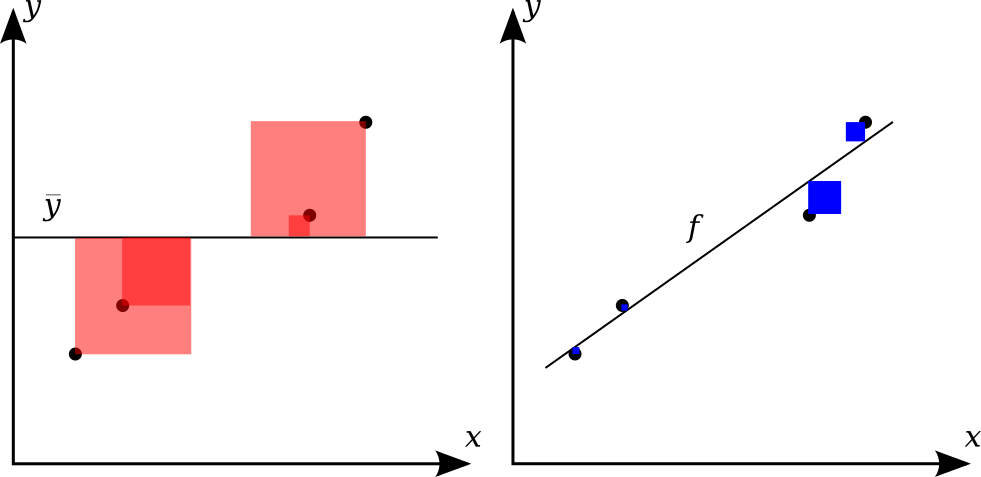
\includegraphics[width=\columnwidth]{./figures/CoD.png}
	\end{center}
\end{figure}
\begin{equation*}
	R^2 = 1 - \frac{\color{blue}{\sum_i (y_i - f(x_i))^2}}{\color{red}{\sum_i (y_i - \bar{y})^2}}
\end{equation*}
As we can see, if the blue term goes to zero, then all the data lie on the line $f(x)$ such that the fit captures the correlation well.
If the blue term goes to infinity, we see that the fit becomes progressively worse and, in this case, $R^2$ becomes negative.


\end{document}
